\documentclass[12pt,a4paper]{standalone}
\usepackage{amssymb}
\usepackage{amsmath}
\usepackage{bm}
\usepackage{tikz}
\usetikzlibrary{arrows.meta}
\usetikzlibrary{arrows}
\usepackage{pstricks}
\usetikzlibrary{patterns}
\usetikzlibrary{fadings}
\usetikzlibrary{shapes.geometric}



\begin{document}
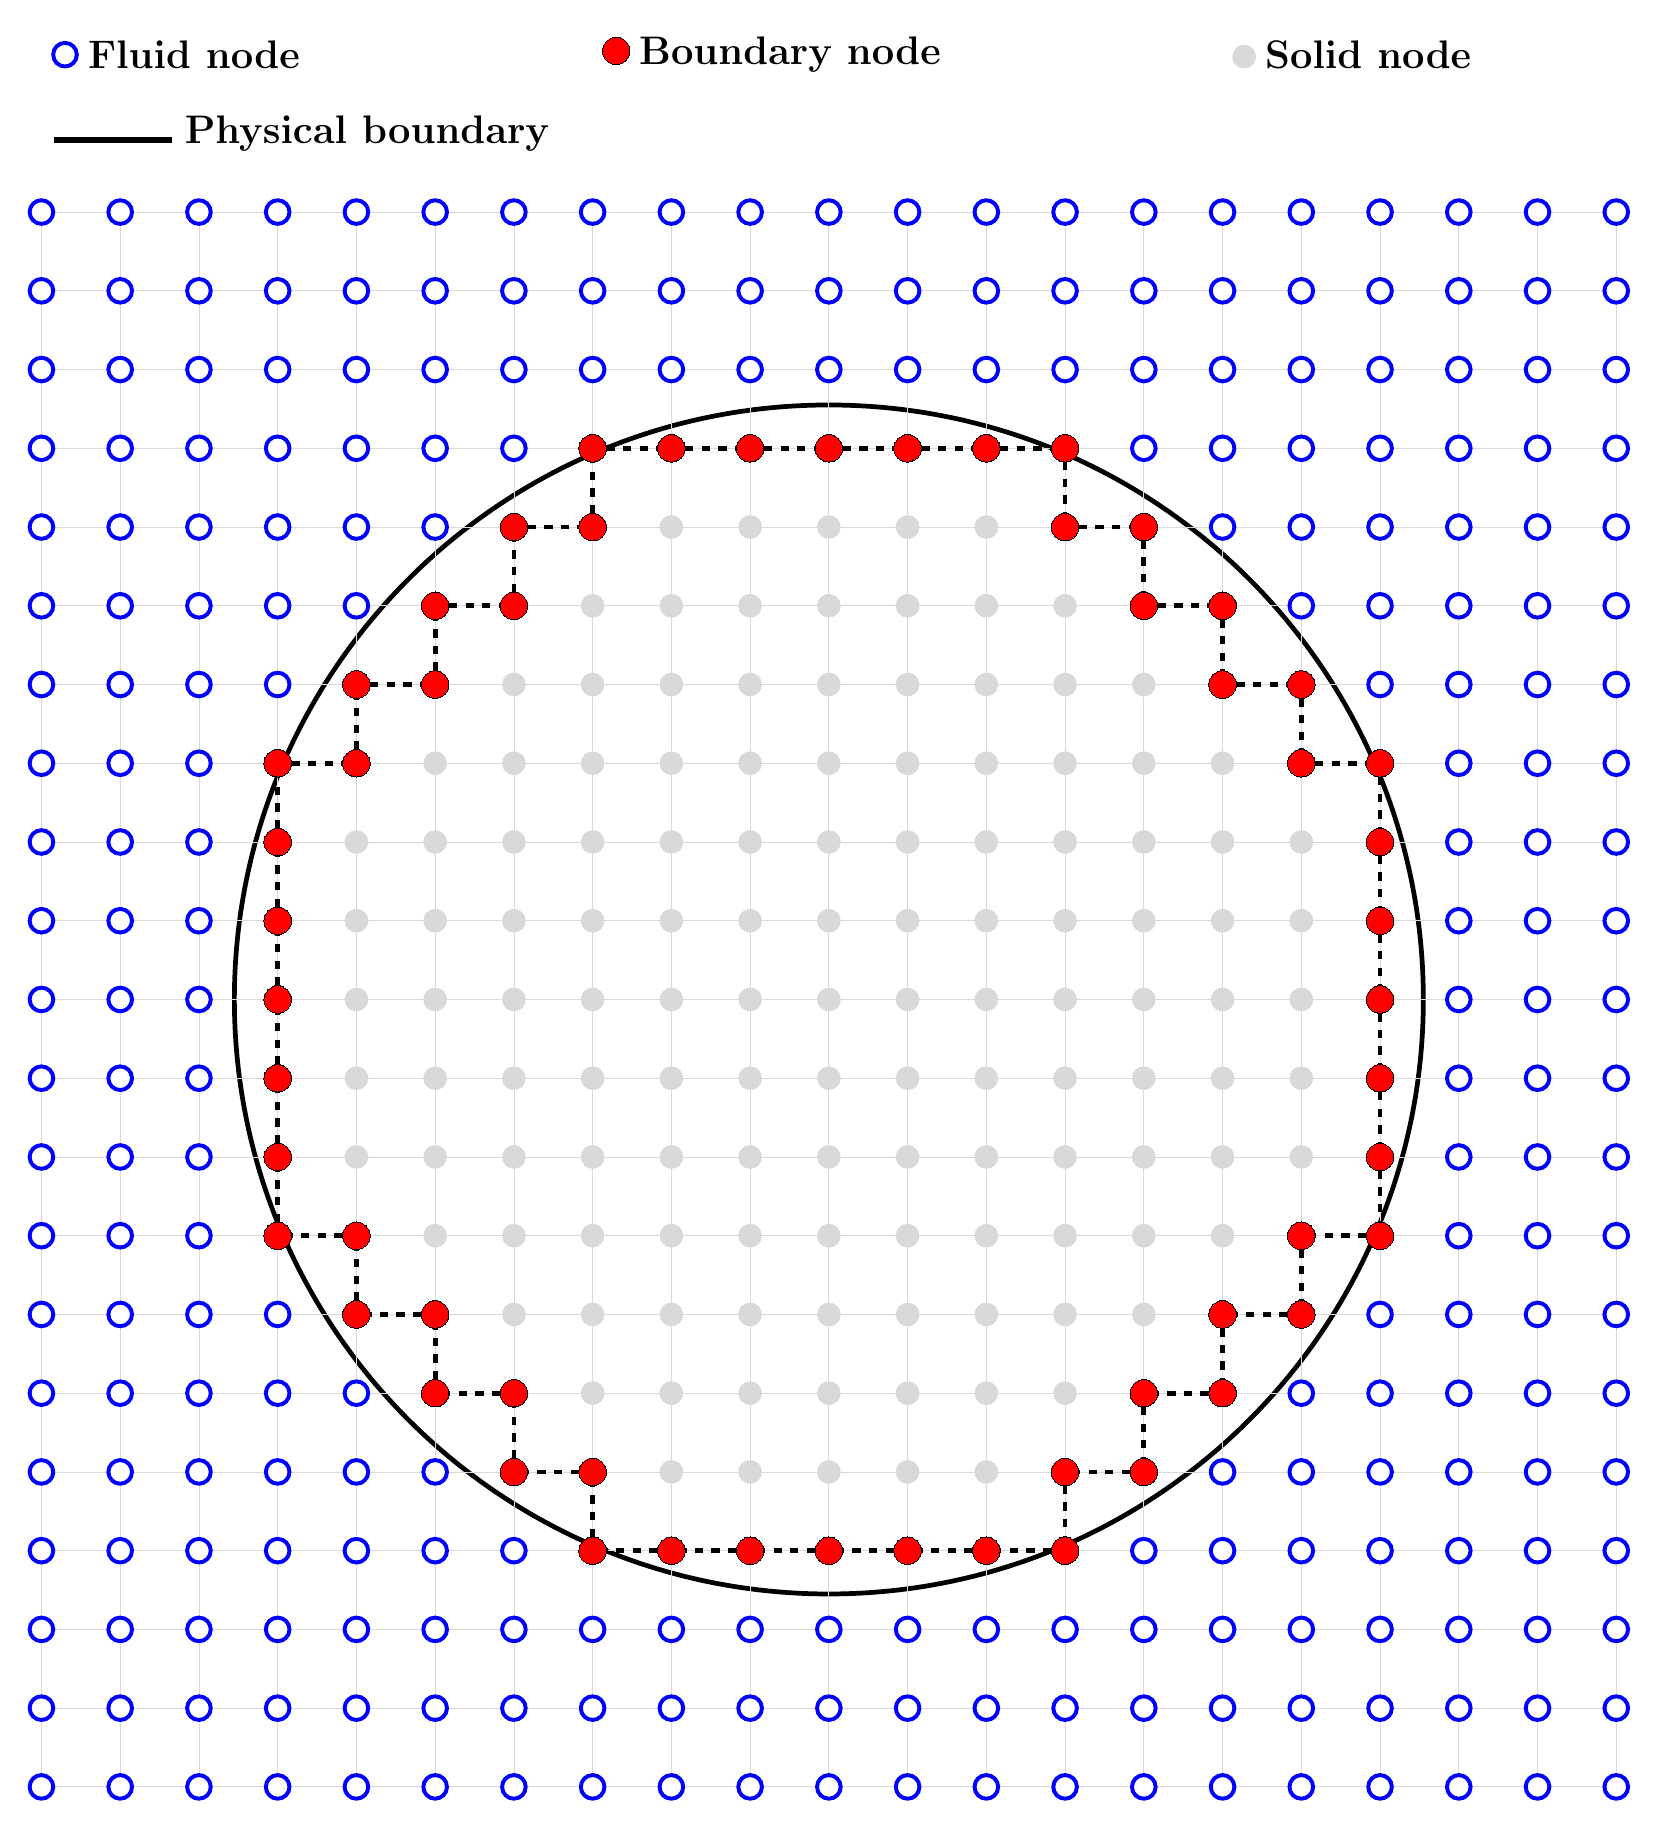
\begin{tikzpicture}[line width=0.6mm]

	%\draw[thick,line width=1mm] (17.5,10) arc[start angle=0, end angle=360, radius=7.53];
	\draw[black,fill=white] (10,10)node[]{} circle(7.55cm);

	\tikzset{myblue/.style={draw=blue, fill=white, line width=0.5mm, circle, minimum size=0.3cm, inner sep=0pt}}

	% Horizontal and vertical grid lines
	\foreach \y in {0,...,20} {
			\draw[gray!30, line width=0.1mm] (0,\y) -- (20,\y);
		}
	\foreach \x in {0,...,20} {
			\draw[gray!30, line width=0.1mm] (\x,0) -- (\x,20);
		}

	% Column 0-2 (full columns)
	\foreach \x in {0,1,2} {
			\foreach \y in {0,...,20} {
					\node[myblue] at (\x,\y) {};
				}
		}

	% Column 3
	\foreach \y in {0,...,6} { \node[myblue] at (3,\y) {}; }
	\foreach \y in {14,...,20} { \node[myblue] at (3,\y) {}; }

	% Column 4
	\foreach \y in {0,...,5} { \node[myblue] at (4,\y) {}; }
	\foreach \y in {15,...,20} { \node[myblue] at (4,\y) {}; }

	% Column 5
	\foreach \y in {0,...,4} { \node[myblue] at (5,\y) {}; }
	\foreach \y in {16,...,20} { \node[myblue] at (5,\y) {}; }

	% Column 6
	\foreach \y in {0,...,3} { \node[myblue] at (6,\y) {}; }
	\foreach \y in {17,...,20} { \node[myblue] at (6,\y) {}; }

	% Column 7
	\foreach \y in {0,...,2} { \node[myblue] at (7,\y) {}; }
	\foreach \y in {18,...,20} { \node[myblue] at (7,\y) {}; }

	% Column 8
	\foreach \y in {0,...,2} { \node[myblue] at (8,\y) {}; }
	\foreach \y in {18,...,20} { \node[myblue] at (8,\y) {}; }

	% Column 9
	\foreach \y in {0,...,2} { \node[myblue] at (9,\y) {}; }
	\foreach \y in {18,...,20} { \node[myblue] at (9,\y) {}; }

	% Column 10
	\foreach \y in {0,...,2} { \node[myblue] at (10,\y) {}; }
	\foreach \y in {18,...,20} { \node[myblue] at (10,\y) {}; }

	% Column 11
	\foreach \y in {0,...,2} { \node[myblue] at (11,\y) {}; }
	\foreach \y in {18,...,20} { \node[myblue] at (11,\y) {}; }

	% Column 12
	\foreach \y in {0,...,2} { \node[myblue] at (12,\y) {}; }
	\foreach \y in {18,...,20} { \node[myblue] at (12,\y) {}; }

	% Column 13
	\foreach \y in {0,...,2} { \node[myblue] at (13,\y) {}; }
	\foreach \y in {18,...,20} { \node[myblue] at (13,\y) {}; }

	% Column 14
	\foreach \y in {0,...,3} { \node[myblue] at (14,\y) {}; }
	\foreach \y in {17,...,20} { \node[myblue] at (14,\y) {}; }

	% Column 15
	\foreach \y in {0,...,4} { \node[myblue] at (15,\y) {}; }
	\foreach \y in {16,...,20} { \node[myblue] at (15,\y) {}; }

	% Column 16
	\foreach \y in {0,...,5} { \node[myblue] at (16,\y) {}; }
	\foreach \y in {15,...,20} { \node[myblue] at (16,\y) {}; }

	% Column 17
	\foreach \y in {0,...,6} { \node[myblue] at (17,\y) {}; }
	\foreach \y in {14,...,20} { \node[myblue] at (17,\y) {}; }

	% Column 18-20 (full columns)
	\foreach \x in {18,19,20} {
			\foreach \y in {0,...,20} {
					\node[myblue] at (\x,\y) {};
				}
		}

	% Boundary nodes with labels p1, p2, ...
	\tikzset{mydot/.style={draw=black, fill=red, line width=0mm, circle, minimum size=0.35cm, inner sep=0pt}}

	% Define and draw nodes
	\node[mydot] (p1) at (3,7) {};
	\node[mydot] (p2) at (3,8) {};
	\node[mydot] (p3) at (3,9) {};
	\node[mydot] (p4) at (3,10) {};
	\node[mydot] (p5) at (3,11) {};
	\node[mydot] (p6) at (3,12) {};
	\node[mydot] (p7) at (3,13) {};

	\node[mydot] (p8) at (4,6) {};
	\node[mydot] (p9) at (4,7) {};
	\node[mydot] (p10) at (4,13) {};
	\node[mydot] (p11) at (4,14) {};

	\node[mydot] (p12) at (5,5) {};
	\node[mydot] (p13) at (5,6) {};
	\node[mydot] (p14) at (5,14) {};
	\node[mydot] (p15) at (5,15) {};

	\node[mydot] (p16) at (6,4) {};
	\node[mydot] (p17) at (6,5) {};
	\node[mydot] (p18) at (6,15) {};
	\node[mydot] (p19) at (6,16) {};

	\node[mydot] (p20) at (7,3) {};
	\node[mydot] (p21) at (7,4) {};
	\node[mydot] (p22) at (7,16) {};
	\node[mydot] (p23) at (7,17) {};

	\node[mydot] (p24) at (8,3) {};
	\node[mydot] (p25) at (8,17) {};

	\node[mydot] (p26) at (9,3) {};
	\node[mydot] (p27) at (9,17) {};

	\node[mydot] (p28) at (10,3) {};
	\node[mydot] (p29) at (10,17) {};

	\node[mydot] (p30) at (11,3) {};
	\node[mydot] (p31) at (11,17) {};

	\node[mydot] (p32) at (12,3) {};
	\node[mydot] (p33) at (12,17) {};

	\node[mydot] (p34) at (13,3) {};
	\node[mydot] (p35) at (13,4) {};
	\node[mydot] (p36) at (13,16) {};
	\node[mydot] (p37) at (13,17) {};

	\node[mydot] (p38) at (14,4) {};
	\node[mydot] (p39) at (14,5) {};
	\node[mydot] (p40) at (14,15) {};
	\node[mydot] (p41) at (14,16) {};

	\node[mydot] (p42) at (15,5) {};
	\node[mydot] (p43) at (15,6) {};
	\node[mydot] (p44) at (15,14) {};
	\node[mydot] (p45) at (15,15) {};

	\node[mydot] (p46) at (16,6) {};
	\node[mydot] (p47) at (16,7) {};
	\node[mydot] (p48) at (16,13) {};
	\node[mydot] (p49) at (16,14) {};

	\node[mydot] (p50) at (17,7) {};
	\node[mydot] (p51) at (17,8) {};
	\node[mydot] (p52) at (17,9) {};
	\node[mydot] (p53) at (17,10) {};
	\node[mydot] (p54) at (17,11) {};
	\node[mydot] (p55) at (17,12) {};
	\node[mydot] (p56) at (17,13) {};

	% Connect boundary with dashed line (main loop)
	\draw[dashed] (p1) -- (p2) -- (p3) -- (p4) -- (p5) -- (p6) -- (p7) -- (p10) -- (p11) -- (p14) -- (p15) -- (p18) -- (p19) -- (p22) -- (p23) -- (p25) -- (p27) -- (p29) -- (p31) -- (p33) -- (p37) -- (p36) -- (p41) -- (p40) -- (p45) -- (p44) -- (p49) -- (p48) -- (p56) -- (p55) -- (p54) -- (p53) -- (p52) -- (p51) -- (p50) -- (p47) -- (p46) -- (p43) -- (p42) -- (p39) -- (p38) -- (p35) -- (p34) -- (p32) -- (p30) -- (p28) -- (p26) -- (p24) -- (p20) -- (p21) -- (p16) -- (p17) -- (p12) -- (p13) -- (p8) -- (p9) -- (p1) -- cycle;

	%Bc fluid
	\tikzset{myblue2/.style={draw=blue, fill=blue, line width=0.5mm, circle, minimum size=0.3cm, inner sep=0pt}}
	\tikzset{mygray/.style={draw=gray!30, fill=gray!30, line width=0.5mm, circle, minimum size=0.25cm, inner sep=0pt}}

	%\node[myblue2] at (3,6) {};
	%\node[myblue2] at (4,5) {};
	%\node[myblue2] at (5,4) {};
	%\node[myblue2] at (6,3) {};
	%
	%\node[myblue2] at (14,3) {};
	%\node[myblue2] at (15,4) {};
	%\node[myblue2] at (16,5) {};
	%\node[myblue2] at (17,6) {};
	%
	%\node[myblue2] at (3,14) {};
	%\node[myblue2] at (4,15) {};
	%\node[myblue2] at (5,16) {};
	%\node[myblue2] at (6,17) {};
	%
	%\node[myblue2] at (17,14) {};
	%\node[myblue2] at (16,15) {};
	%\node[myblue2] at (15,16) {};
	%\node[myblue2] at (14,17) {};

	\foreach \y in {8,...,12} { \node[mygray] at (4,\y) {}; }
	\foreach \y in {7,...,13} { \node[mygray] at (5,\y) {}; }
	\foreach \y in {6,...,14} { \node[mygray] at (6,\y) {}; }
	\foreach \y in {5,...,15} { \node[mygray] at (7,\y) {}; }
	\foreach \y in {4,...,16} { \node[mygray] at (8,\y) {}; }
	\foreach \y in {4,...,16} { \node[mygray] at (9,\y) {}; }
	\foreach \y in {4,...,16} { \node[mygray] at (10,\y) {}; }
	\foreach \y in {4,...,16} { \node[mygray] at (11,\y) {}; }
	\foreach \y in {4,...,16} { \node[mygray] at (12,\y) {}; }
	\foreach \y in {5,...,15} { \node[mygray] at (13,\y) {}; }
	\foreach \y in {6,...,14} { \node[mygray] at (14,\y) {}; }
	\foreach \y in {7,...,13} { \node[mygray] at (15,\y) {}; }
	\foreach \y in {8,...,12} { \node[mygray] at (16,\y) {}; }

	\draw (0,22) node[anchor=west] { \tikz{\node[myblue] {};} {\Large\textbf{Fluid node} }};
	\draw (7,22) node[anchor=west] { \tikz{\node[mydot] {};} {\Large\textbf{Boundary node} }};
	\draw (15,22) node[anchor=west] { \tikz{\node[mygray] {};} {\Large\textbf{Solid node} }};
	%\draw (0,21) node[anchor=west] { \tikz{\node[myblue2] {};} {\Large\textbf{Fluid node with missing neighbour} }};
	\draw (0,21) node[anchor=west] { \tikz{\draw[black,thick, line width=0.8mm] (0,0.8) -- (1.5,0.8);} {\Large\textbf{Physical boundary}} };

\end{tikzpicture}

\end{document}

